\documentclass{article}
\usepackage{graphicx}
\usepackage[utf8]{inputenc}
\usepackage{listings}
\usepackage{color}
\usepackage{upquote}

\definecolor{bluekeywords}{rgb}{0.13,0.13,1}
\definecolor{greencomments}{rgb}{0,0.5,0}
\definecolor{redstrings}{rgb}{0.9,0,0}

 
\lstdefinelanguage{FSharp}%
{morekeywords={let, override, new, match, with, rec, open, module, namespace, type, of, member, % 
and, for, while, true, false, in, do, begin, end, fun, function, return, yield, try, %
mutable, if, then, else, cloud, async, static, use, abstract, interface, inherit, finally },
  otherkeywords={ let!, return!, do!, yield!, use!, var, from, select, where, order, by },
  keywordstyle=\color{bluekeywords},
  sensitive=true,
  basicstyle=\ttfamily,
	breaklines=true,
  xleftmargin=\parindent,
  aboveskip=\bigskipamount,
	tabsize=4,
  morecomment=[l][\color{greencomments}]{///},
  morecomment=[l][\color{greencomments}]{//},
  morecomment=[s][\color{greencomments}]{{(*}{*)}},
  morestring=[b]",
  showstringspaces=false,
  literate={`}{\`}1,
  stringstyle=\color{redstrings},
}

\title{10g rapport}
\author{Henrik Flindt\\Nicolas Dyhrman\\Adrian Joensen}
\date{\today}

\begin{document}
    \maketitle
    
    \section{Wolf in Moose's Clothing}
    \textit{"A single type of bird can be called a goose, but more is geese, but the plural of moose is not meese, and finally one wolf becomes several wolves. English is like coding. Nobody really know why we do it that way we do, but people on the internet will yell at you for getting it wrong."} \newline -Based on common saying. \newline \newline
    The main assignment is the creation of a game, that mimic the relations between mooses and wolfs in a closed park. Each iteration of the game will see the animals move, reproduce and potentially eat a moose. The game is played from the command line interface, by calling its main function called \verb|experimentWAnimals.exe| and give it eight arguments, that fits with the assignment specifications. If done correct, afther the program has run its cause a text file is created with information about the game. 
	\section{Problem Analysis}
	The overall problem is keeping track of two similar but distinct types, and their placement in a 2D array.  To do this several control features must be implemented. The key words of move, reproduce, and eat, combined with the validity of these must be in focus. 

    \section{Design}
    	The overall sourcecode lay out is based upon the one given as part of the assigment, except the environment. To that the behaviors and events were added. 
    
   
   
    \subsection{Two-lists makes a board}
    The board contains two lists, one for each animal type. Any update to animal position and number of animals is checked in comparison with the board width.  
    \subsection{Animals}
    Animals are objects with properties symbol, position, reproduction. Symbol contains a character, either 'm', 'w' or ' ', and is used to identify the animal. Position contains either Some(int * int) or None, and is the position of the board. Reproduction contains an integer and is used to indicate when it is time to reproduce.
    \\
    Animals also has behaviours called updateReproduction() and resetReproduction(). The former reduces the reproduction property by 1, and the latter resets it to the start value.
     To move the animals, a random vector was pick based upon a random number from 0 to 7 (There are a total of 3x3-1 = 8 directions), where the direction was check if it's a valid, and if so change the animals' position with the vector.\newline
    To make the order of animals random, first the wolf list is selected and a tuole list is create a tuple list, where the first element will contain their symbol "w" and the second element will contain the index of the wolves. This is also done to the moose list. This is done for the entirety of the two lists, which are then joined and shuffled. \newline To shuffle the tuple list, a function with a for loop was used. It picks a random index, remove the element from the tuple list and put it in a new list. When the tuple is empty, the new list is returned.. After this shuffle, this tuple is used to deside the order of succession. \newline	
    
    \subsubsection{Wolf}
    	Wolf inherits Animals, but has one more attribute hunger and many additional methods, updateHunger(), resetHunger() and tick(). Hunger is used to tell when it's time to hunt or die. updateHunger() reduces the hunger by 1 and changes position to None if hunger is 0. resetHunger() resets hunger to start value. tick() returns either a wolf object or None. 
    The wolves ability to eat a moose was implemented specifically for them, and works in a similarly as the move function, but with mooses being a favored direction compared to a empty or wolf occupied location. If the wolf sees one or more mooses next to it, it will pick one at random and move there. The moose is noted as dead and removed later.  
    
    
    \subsubsection{Moose}
    	Moose inherits Animals, but has an additional method, tick(), which returns a Moose object or None.

    \section{Implementation}
        \subsection{Manual}
    To compile the main function, type: \newline \verb|fsharpc animalsSmall.fs experimentWAnimals.fsx|\newline
    To run the main function, type: \newline \verb|mono experimentWAnimals.exe tic file.txt size moose fMoose wolf fWolf hWolf|\newline
    \verb|tic| is the integer amount of iterations the game will run. \verb|file.txt| is the name of the file where the data shall be saved. Must end with \verb|.txt|. \verb|size| is the size of the squared board. \verb|moose|
    and \verb|wolf| is the amount of the two animals respectively. \verb|fmoose| and \verb|fWolf| is the time interval in tics, of where the two different animals shall multiply. Finally \verb|hWolf| is when a wolf ought to eat to avoid starvation and death.\newline \newline
    To compile the whitebox test, type: \newline \verb|fsharpc animalsSmall.fs whiteboxtest.fsx|\newline
    To run the whitebox test, type: \newline \verb|mono whiteboxtest.exe|\newline
    
     \subsection{Main function and its arguments}
    The main function was designed to sanitize the user input, and only allowing valid inputs. First it is checked if all the inputs are eighter integers, or in the case of the second argument, a string containing ".txt" in it. \newline Afterwards several minimum values was implemented, no max values were chosen. While this could be valid as to avoide overflows, all functions works on the premise of list, and thus overflow could only occur if it is an int32 overflow. Since the program begins to take prolonged time when the animal count increases, it is believed that this overflow risk is minimal in a human lifetime. All integer values give (except for the tick int) must be above 0. \newline While the code can handle 0 animals, a follow effect is that the other values then also should be zero. It was decided to solve this problem with avoiding it. As for the final tick int that can be all the subsets of integers, it is used to check that first round placement (i.e tick = 0) is random, and that a fil is always created (tick < 0 ).\newline The overall design is a row of if-statments. It's a simple code, but quite effective. 

         
\section{Whitebox testing}
    \subsection{moose.tick}
    moose.tick went as expected and only gave us an option if the mooses $repLen$ was 0 or under. And otherwise gave us a None as it was not ready.
    
    \subsection{wolf.tick}
    wolf.tick went as expected and only gave us an option if the wolfs $repLen$ was 0 or under. And otherwise gave us a None as it was not ready.
    
    \subsection{enviroment.genMoveVector}
    The general move functions was visually tested on single animals setup, with a low reproduction and hunger rate. This is due to the random nature of the movements, and the overall visual aspect of the movement. It was discovered that several animals, that could reproduce, sometimes appeared not to move. This is believed to be a false negative test, caused by the animals moving at random in synchronization fo a single iteration. Therefor the test was done with a higher level of manual control. \newline
    
    \subsection{enviroment.moveAnimal}
    moveAnimal went as expected and gave us the answers we expected.
    
    \subsection{enviroment.countMoose}
    The method went as expected and counted all the living mooses in the system.
    
    \subsection{enviroment.countWolfs}
    The method went as expected and counted all the living wolfs in the system.
    
    \subsection{enviroment.checkForAnimalsAtPosition}
    the method went as expected, and send a bool back wether there was animals at the specific position
    
    \subsection{enviroment.checkValidMove}
    The method went as expected, and send back a bool of wether the move the animal wanted to do, is a valid move.
    
    \subsection{enviroment.findMooseAtPosition}
    The method went as expected, and send back a bool of wether there was a moose at this position or not.
    
    \subsection{enviroment.checkFieldsAround}
    The method went as expected, and checked wether there was any valid moves around the given position
    
    \subsection{enviroment.CheckEating}
    The method went as expected, and sent back a generic list of all the the positions where there would be a moose.
    
    \subsection{enviroment.KillMooseFromPosition}
    The method went as expected, and made the moose at that position's, position to be None.
    
    \subsection{enviroment.removeDeadAnimals}
    The method went as expected, and killed all animals whom's position was None.
    
    \subsection{enviroment.tick}
    This method just called 2 others and therefore we didnt see the nessecarity of us actually testing it.
    
    \subsection{enviroment.makeQueue}
    Since this works by putting in all of them by random in random places, we have just displayed them, and looked that they were not the same, and that every animal was in the scrambled list. Also checked that they were scrambled different that the other 2 that we made.
    
    \subsection{WriteOutInfo}
    Since this is basicly the same as the function made for us, but with some text on it we assume it will still work, as assumed when it was given to us. Also tested while looking at our runs of our program.
    
    \section{Experiment}
    For the experimental analysis, the success criteria was a substaniable population of both animals, with non-dying out. Secondely while the mooses can survive without wolfs, they would take up all room on the board. This is seen as a negative in this case. \newline
    While this experiment could be a multi-variable experiment, with free ranging variables, it was decided to lock iterations at 15, board at 10 and varier the final 5 variabels between a low of 2 and a high of 10. Futher more it was decided to fits this to a reduced 2-to-the-k-factorial experiment. (Otherwise had it not been reduced it would have been 2 to the power of 5 would give 32 x 15 480 data points to collect.) The reduction was set to 10 tests. 
    
    \begin{figure}[]
    	\centering
    	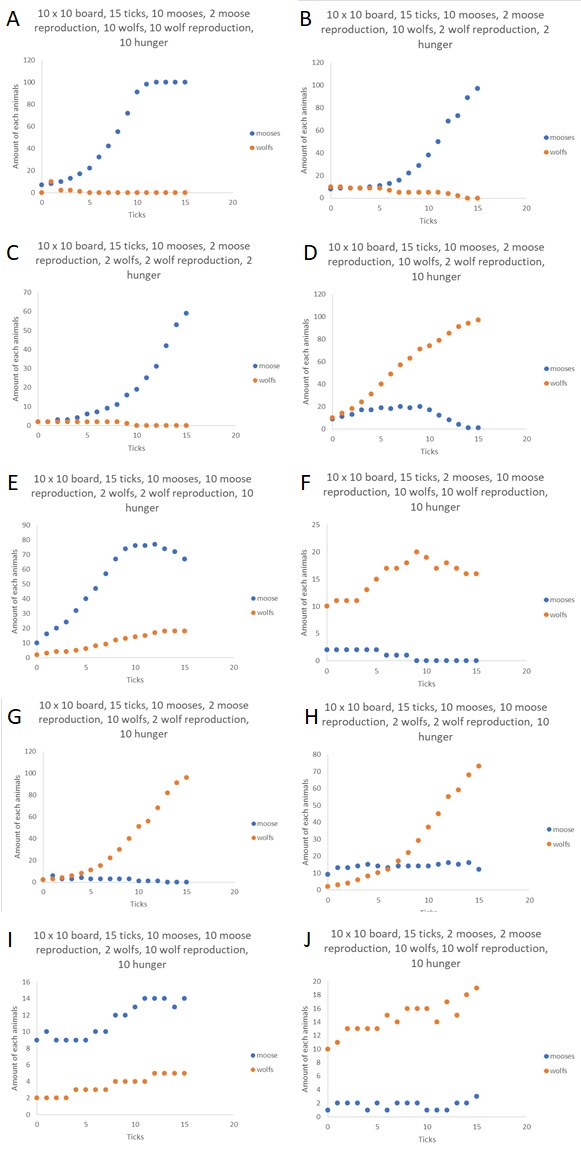
\includegraphics[scale=0.6]{./rawdata.jpg}	
    \end{figure}
    
        It is clealry seen that a natural plato is reached when no inhibition is reached. This is quite similar to Michaelis–Menten kinetics as seen in enzyme kinetivs. It follow a v = d[P]/dt = Vmax[S]/(Km +[S]) formular of transformation. In this case with no inhibition (i.e. low wolfs) the moose population changes empty space (S) to moose (P). Km is halfway point between the lowest and highest population of mooses. The few iterations prior to the higher plato (figure A around iteration 10), is caused by a lack of space. In the rapid growing interval the mooses have room to reproduce, but in the final stage the odds of a reproducing moose having room becomes smaller and the rate drops. \newline
        
        When there is inhibition seen it can be seen that the rate of each animal never	 reaches a true steady plato (As in figure J), since an over abundance of wolfs begins to die, causing remaining mooses to grow till the large population of wolfs reduces this again. \newline
        
       
        
        Over all the two best combinations for keeping a stable population of thw two is seen in figure E and I, where a large moose population reproduce enough to keep a small group of wolfs alive, but without reaching the palto seen in figure A, where the mooses are to numerous for the space given.  This is a good starting point to fine tune any given population of wolfs and mooses. A truely perfect setup might not be truely reached withing the first few hundred iteratios, due to the random nature of the setup, but with the parameters in figure I and E a well-informed estimate can be made with a few set of extra experiments. A high mooses population might also be needed to avoide a situationas in figure F, which is quite similar to I and E but with a small moose population to start with.
        
    \section{Conclusion}
     While the program functions as expected, it does increase a disproportionate amount when the animal count or board size increases. This is believed to be cause by the high amount of lists being used to keep track of the animals. Each time an animal makes a move it checks the entire list as to ensure no animal is next to it. This ramification due to the design, was to monumental to redesign when discovered, but should be fixed in the case of more widespread use. \newline
     Based upon the data gathered in 10 experiments it can be concluded that the birth rate of the mooses must be proportionate to the wolfs hunger, and but with a potential higher stating population of mooses. 
     
 

\end{document}
